% !TEX program = pdflatex
% English version — compiles with pdfLaTeX (default on Overleaf, no Chinese font needed)
\documentclass[11pt,a4paper]{article}

\usepackage[utf8]{inputenc}
\usepackage{amsmath,amssymb}
\usepackage{booktabs}
\usepackage{array}
\usepackage{graphicx}
\usepackage{hyperref}
\usepackage[margin=2.5cm]{geometry}
\usepackage{enumitem}
\usepackage{url}

\hypersetup{colorlinks=true, linkcolor=blue, citecolor=blue, urlcolor=blue}

\title{\textbf{Graph-Constrained Reasoning with Bidirectional\\Sub-Answer Verification for Multi-Hop QA}}
\author{zhouduomu}
\date{}

\begin{document}
\maketitle

\begin{abstract}
Existing graph-enhanced reasoning methods model inference as a DAG, yet their consistency checks rely on pure graph-theoretic structural metrics (connectivity, acyclicity, coverage) that cannot reflect reasoning correctness. As a result, the Consistency Score provides little discriminative signal between correct and incorrect reasoning, and multi-path selection degenerates into random sampling. We propose GERS, which models reasoning as a dependency DAG executed in topological order. The core contribution is \textbf{bidirectional sub-answer verification}: using the final answer and context as an anchor, each sub-question is re-derived in reverse and the forward/backward sub-answers are compared, upgrading the Consistency Score from a structural-validity metric into a content self-consistency signal. On 500 HotpotQA samples, this raises the score's correct/wrong discrimination from $-0.0035$ to $+0.0847$; the best configuration GERS-CV2 achieves EM=0.302, F1=0.413, improving over CoT-SC by 4 F1 points, with a significant McNemar test on EM correctness ($p=0.029$) but marginal paired bootstrap effect-size intervals. We further provide a boundary analysis on 2WikiMultiHopQA, showing the method suits comparison-style decomposition but fails on deep bridge-comparison questions where upstream entity errors propagate.
\end{abstract}

\noindent\textbf{Keywords:} Large Language Models; Multi-hop Reasoning; Chain-of-Thought; Graph Representation; Bidirectional Cross-Validation; Consistency Verification

\section{Introduction}

Multi-hop reasoning requires models to combine evidence across multiple fragments, and is a core task for evaluating LLM reasoning ability. Chain-of-Thought (CoT) prompting~\cite{wei2022cot} significantly improves LLM performance by eliciting intermediate steps. However, standard CoT organizes reasoning as \textbf{linear text}, with two key limitations:

\begin{enumerate}[label=\arabic*.]
\item \textbf{Missing non-linear dependencies}: CoT strings steps linearly and cannot express branching, merging, or parallel dependencies among sub-questions. When the reasoning path is inherently a DAG rather than a chain, linearization loses structural information.
\item \textbf{Quality-agnostic voting}: CoT-SC~\cite{wang2023sc} samples multiple paths and takes the majority answer, but votes are equal-weighted and cannot exploit the quality of each reasoning path.
\end{enumerate}

Recent works enhance reasoning with graph structures: GoT~\cite{besta2024got} proposes graph-of-thoughts with merging/distillation but does not guarantee execution order; RwG~\cite{han2025rwg} structures context into an entity-relation graph but does not execute step-by-step; MoDeGraph~\cite{oruche2025modegraph} builds a multi-hop dependency graph but remains a prompt method without topological execution or consistency checking. These methods treat the graph as a prompt decoration or post-hoc verification, rather than a component that participates in execution and quality assessment---more critically, \textbf{none of them uses graph-structure quality to guide answer selection}.

To address this, we propose \textbf{GERS}, which explicitly models reasoning as a dependency DAG executed in topological order. We find that computing a Consistency Score purely from graph-theoretic properties is ineffective: LLM-generated decomposition graphs are almost always legal DAGs, so scores cluster (around 0.6--0.7) and multi-path selection degenerates to random sampling (measured discrimination only $-0.0035$ on 500 samples). We therefore propose the core innovation \textbf{bidirectional sub-answer verification}: using the final answer and context as an anchor, each sub-question is re-derived in reverse and the forward/backward sub-answers are compared, upgrading the Consistency Score from a structural-validity metric into a content self-consistency signal. This verification is naturally supported by explicit DAG decomposition---which provides named sub-question units and dependency edges---and is less straightforward to apply to unstructured linear CoT outputs.

Rather than claiming uniform superiority over all prompting baselines, this work identifies and fixes a key bottleneck of graph-based reasoning: structural graph validity is not equivalent to reasoning correctness. Our contributions are organized in three layers:
\begin{enumerate}[label=\arabic*.]
\item \textbf{Mechanism contribution (core)}: Bidirectional sub-answer verification raises the Consistency Score's correct/wrong discrimination from $-0.0035$ to $+0.0847$ (500 HotpotQA samples), turning consistency checking from a structural metric into an effective content self-consistency signal.
\item \textbf{Empirical contribution}: The best configuration GERS-CV2 achieves EM=0.302, F1=0.413 on HotpotQA (500 samples), with a significant McNemar test on EM correctness (McNemar $p=0.029$) and a +4pt F1 difference over CoT-SC, though with marginal paired bootstrap effect-size intervals that we report transparently.
\item \textbf{Diagnostic contribution}: We provide a boundary analysis on 2WikiMultiHopQA, showing the method suits comparison-style decomposition but fails on deep bridge-comparison questions where upstream entity errors propagate. We also report that graph-level multi-path self-consistency yields no extra gain on medium-difficulty multi-hop even after fixing CS discrimination.
\end{enumerate}

\section{Related Work}

\noindent\textbf{Chain-of-Thought reasoning.} Wei et al.~\cite{wei2022cot} proposed CoT prompting. Wang et al.~\cite{wang2023sc} proposed Self-Consistency (CoT-SC), whose equal-weight voting does not exploit path quality. Yao et al.~\cite{yao2023tot} proposed Tree of Thoughts (ToT), with no explicit dependency modeling among sub-questions. These methods are based on linear or tree structures.

\noindent\textbf{Graph-enhanced reasoning.} GoT~\cite{besta2024got} models reasoning as a graph for merging/distillation but focuses on prompt engineering. RwG~\cite{han2025rwg} uses a context graph as a one-time input. MoDeGraph~\cite{oruche2025modegraph} builds a multi-hop dependency graph but remains a prompt method. StepChain~\cite{ni2025stepchain} combines decomposition with BFS but uses a linear sequence rather than a DAG. GERS deeply couples the reasoning graph with execution and uses graph-structure quality as a selection signal.

\noindent\textbf{Verification and consistency checking.} Process Reward Models~\cite{lightman2024verify} score intermediate steps but require large amounts of labeled data. Self-Refine~\cite{madaan2023selfrefine} iteratively refines answers via self-feedback but operates on linear text without a verifiable sub-question structure. GERS uses graph-theoretic algorithms for structural checking and designs bidirectional sub-answer verification so that checking directly affects the final answer.

\section{Method}

\subsection{Overall Framework}

GERS has three modules: reasoning-state graph representation, graph-constrained chain generation, and consistency checking. The flow (Figure~1): input $Q,C$ $\to$ ① decompose into sub-questions $\{q_i\}$ with dependencies $\to$ ② build DAG $G=(V,E)$ $\to$ ③ topological sort $\tau$ $\to$ ④ execute step-by-step to get sub-answers $a_i$ $\to$ ⑤ aggregate into final answer $A$ (answer-type alignment) $\to$ ⑥ consistency check $S = 0.3\cdot S_{\text{struct}} + 0.7\cdot S_{\text{crossval}}$ $\to$ (GERS-SC: select the best of $K$ DAGs) $\to$ output $A, G, S$.

\begin{figure}[h]
\centering
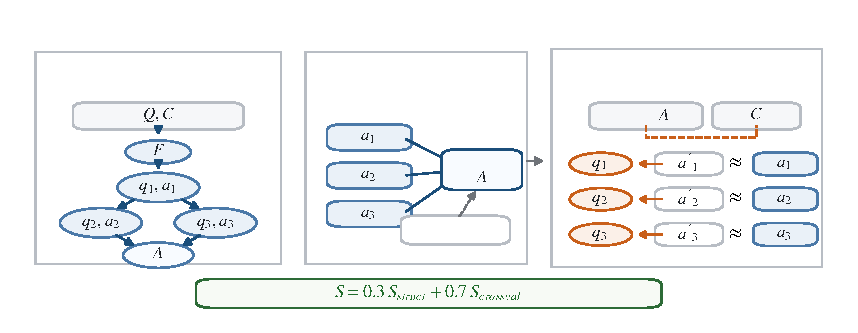
\includegraphics[width=0.85\textwidth]{figures/image1}
\caption{GERS reasoning framework. The model decomposes a question into a dependency DAG, executes sub-questions in topological order, aggregates a final answer, and performs bidirectional sub-answer verification anchored by the final answer and context.}
\end{figure}

\subsection{Reasoning-State Graph Representation}

Nodes: FactNode (facts/original question), StepNode (sub-question and answer), ConclusionNode (final conclusion). Edges: DeriveEdge ($u\to v$), SupportEdge, ConflictEdge. The LLM decomposes $Q$ into an ordered sub-question list with dependencies, and nodes/edges are created accordingly.

\subsection{Graph-Constrained Chain Generation}

\textbf{Path planning.} Topological sort gives execution order $\tau=(v_1,\dots,v_n)$; cycles are broken first. Each sub-question is answered only after its predecessors.

\textbf{Execution and aggregation.} Sub-questions are answered in topological order, with each answer passed as context to dependent sub-questions (dependency propagation). The reasoning chain is aggregated into the final answer $A$.

\textbf{Answer-type alignment.} The final answer must match the entity type requested by the original question (e.g., if the question asks ``which film'', the answer must be a film name, not an intermediate director). This is critical for bridging-comparison questions.

\subsection{Consistency Checking and Bidirectional Cross-Validation}

\textbf{Structural Consistency Score (baseline).}
\begin{equation}
S_{\text{struct}} = w_1\cdot C_{\text{conn}} + w_2\cdot C_{\text{cycle}} + w_3\cdot C_{\text{cov}}
\end{equation}
with $w_1=w_3=0.35, w_2=0.30$ for connectivity, acyclicity, and coverage, plus a chain-length penalty.

\textbf{Limitation of the structural layer.} LLM-generated graphs are almost always legal connected acyclic DAGs, so $S_{\text{struct}}$ clusters (mean 0.662, std 0.098, discrimination $-0.0035$) and cannot distinguish reasoning quality.

\textbf{Sub-answer bidirectional cross-validation (core).} Given forward sub-answers $\{a_i\}$ and final answer $A$, each sub-question is re-answered in reverse using ``final answer $A$ + context $C$'' as the anchor, yielding backward sub-answers $\{a'_i\}$; consistency is then:

\begin{figure}[h]
\centering
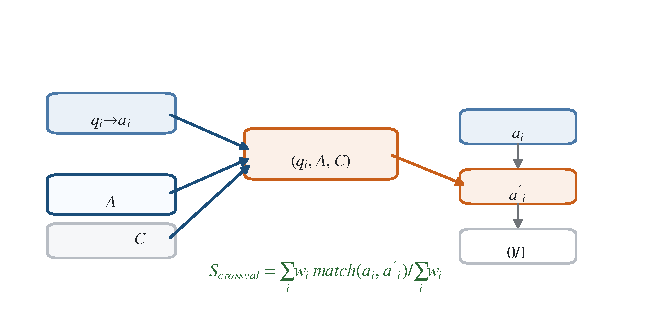
\includegraphics[width=0.85\textwidth]{figures/image3}
\caption{Bidirectional sub-answer verification. Given forward sub-answers and the final answer, each sub-question is re-derived in reverse from the answer+context; forward/backward agreement yields a content self-consistency score that replaces the non-discriminative structural score.}
\end{figure}
\begin{equation}
S_{\text{crossval}} = \frac{\sum_{i=1}^{n} w_i\cdot\mathbb{1}[\text{match}(a_i, a'_i)]}{\sum_{i=1}^{n} w_i}
\end{equation}
where the weight $w_i = 0.5 + 0.5\cdot(i+1)/n$ gives downstream sub-questions (later in the topological order) higher weight, as their errors propagate further. The match function is a three-level heuristic: (i) \emph{exact match} after normalization (lowercasing, punctuation removal, yes/no and numeric unification) returns 1; (ii) \emph{substring containment} or numeric equality returns 1; (iii) otherwise 0. An optional LLM judge (disabled by default for cost) can be enabled for residual semantic cases. The reverse prompt explicitly requires ``re-derive from the context, do not copy the final answer'' to mitigate confirmation bias. This verification is naturally supported by explicit DAG decomposition---which provides named sub-question units and dependency edges---and is more direct and interpretable than applying it to unstructured CoT text.

\textbf{New Consistency Score.} The structural and content layers are combined with fixed weights (set heuristically and held constant across all experiments, without test-set tuning):
\begin{equation}
S = 0.3\cdot S_{\text{struct}} + 0.7\cdot S_{\text{crossval}}
\end{equation}

\subsection{Sub-Answer Confidence-Weighted Aggregation}

Each sub-answer confidence is estimated by a lightweight heuristic (no extra LLM call), considering non-emptiness, absence of uncertainty signals, entity grounding in context, and whether it is a pure number. Sub-answers below threshold $\theta_{\text{conf}}=0.5$ are tagged \texttt{[LOW CONFIDENCE]} in the aggregation prompt, reducing single-step error propagation.

\subsection{Graph-Level Self-Consistency (GERS-SC)}

GERS-SC generates $K$ DAGs (decomposition temperatures $T\in\{0.3,0.5,0.7\}$) and selects the highest-scoring one: $A^*=\arg\max_k S(G_k)$. Bidirectional cross-validation is designed to make this score-based selection meaningful by improving CS discrimination, although experiments below show that multi-path selection still yields limited end-task gains.

\section{Experiments}

\subsection{Setup}

\textbf{Datasets.} HotpotQA~\cite{yang2018hotpotqa} (500 samples: 404 bridge + 96 comparison); 2WikiMultiHopQA~\cite{ho20202wiki} (100 samples: comparison/bridge\_comparison/compositional/inference).

\textbf{Baselines.} Zero-Shot, Standard CoT, CoT-SC ($N=3$), CoT-SC+GERS rerank (ablation). All methods use a unified concise answer extraction and normalization pipeline.

\textbf{Our methods.} GERS+adaptive (DAG execution + adaptive routing); GERS-SC (+graph-level self-consistency $K=3$); GERS-CV (+bidirectional cross-validation); GERS-CV2 (+confidence weighting, best).

\textbf{Model.} Qwen3-8B (DashScope API), 4-worker parallel, zero failures. \textbf{Metrics:} EM, F1, Consistency Score. Main comparisons report paired bootstrap 95\% CIs (10000 resamples) for EM/F1 differences and McNemar tests for paired EM correctness.

\textbf{Evaluation fairness.} To avoid evaluation-pipeline distortions, we unify three treatments: (1) fix the EM bidirectional-substring bug (which inflated numeric answers); (2) unified concise extraction/normalization for all methods; (3) answer-type alignment in GERS aggregation. This ensures all methods are compared on the same fair footing, so any GERS gain comes from the method itself.

\subsection{Main Results}

\begin{figure}[h]
\centering
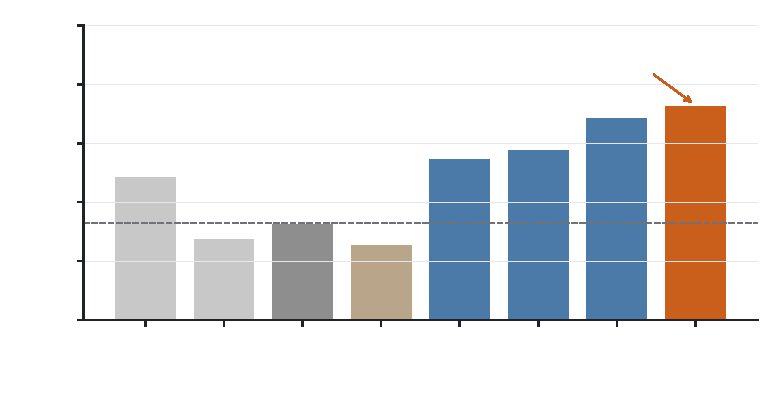
\includegraphics[width=0.85\textwidth]{figures/image4}
\caption{Main F1 results on HotpotQA (n=500). GERS-CV2 achieves the highest F1; the annotation reports the paired bootstrap interval for the F1 difference against CoT-SC.}
\end{figure}

\begin{table}[h]
\centering
\caption{Main results (HotpotQA, n=500)}
\resizebox{\linewidth}{!}{%
\begin{tabular}{lccc}
\toprule
Method & EM & F1 & CS \\
\midrule
Zero-Shot & 0.276 & 0.389 & --- \\
Std CoT & 0.264 & 0.368 & --- \\
CoT-SC (N=3) & 0.262 & 0.373 & --- \\
CoT-SC+GERS rerank & 0.264 & 0.372 & --- \\
GERS-Adap. & 0.284 & 0.395 & 0.996 \\
GERS-SC (K=3) & 0.282 & 0.398 & 0.662 \\
GERS-CV (+verification) & 0.298 & 0.409 & 0.782 \\
\textbf{GERS-CV2 (+confidence)} & \textbf{0.302} & \textbf{0.413} & 0.777 \\
\bottomrule
\end{tabular}}
\end{table}

GERS-CV2 achieves the best EM=0.302 and F1=0.413, with a +4pt F1 difference over CoT-SC and a paired-significant McNemar test on EM correctness. Bidirectional verification (0.284$\to$0.298) contributes +1.4pt EM---the direct gain of the core innovation. The CoT-SC+GERS rerank variant (0.372) is on par with CoT-SC (0.373), indicating that applying graph scores post hoc to already-generated linear CoT answers is insufficient; the graph must participate in generation and verification rather than merely reranking. Note Zero-Shot (0.276) is already close to GERS on HotpotQA; we analyze this in Section~4.4.

\begin{table}[h]
\centering
\caption{Significance tests (HotpotQA, n=500). EM/F1 differences report paired bootstrap 95\% CIs (10000 resamples); McNemar $p$ is computed on paired EM correctness.}
\resizebox{\linewidth}{!}{%
\begin{tabular}{lccccc}
\toprule
Comparison & EM diff & EM 95\% CI & F1 diff & F1 95\% CI & McNemar $p$ \\
\midrule
GERS-CV2 vs CoT-SC & +0.040 & [$-0.014, +0.096$] & +0.041 & [$-0.014, +0.095$] & \textbf{0.029} \\
GERS-CV2 vs Std CoT & +0.038 & [$-0.018, +0.094$] & +0.045 & [$-0.009, +0.099$] & \textbf{0.040} \\
GERS-SC vs CoT-SC & +0.020 & [$-0.034, +0.076$] & +0.025 & [$-0.029, +0.079$] & 0.275 \\
\bottomrule
\end{tabular}}
\end{table}

GERS-CV2 yields a significant paired McNemar test against CoT-SC on EM correctness ($p=0.029$), but the paired bootstrap 95\% CIs for the EM and F1 differences marginally cross zero (lower bound $\approx -0.014$). We transparently report this as a ``paired-significant on correctness, effect-size marginal'' result rather than claiming strong significance. By contrast, GERS-SC without verification ($p=0.275$) is not significant, corroborating that the gain stems from bidirectional verification.

\subsection{Repairing Consistency Score Discrimination (Core Evidence)}

\begin{figure}[h]
\centering
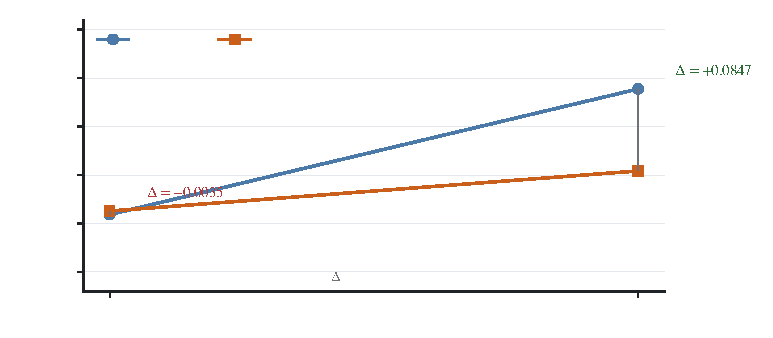
\includegraphics[width=0.8\textwidth]{figures/image2}
\caption{Consistency Score discrimination (HotpotQA, n=500). The old structural CS clusters around 0.66 for both correct and wrong answers (discrimination $-0.0035$); the new CS with bidirectional verification separates them (discrimination $+0.0847$), measured on the GERS-CV variant.}
\end{figure}

\begin{table}[h]
\centering
\caption{CS correct/wrong discrimination (HotpotQA, n=500)}
\begin{tabular}{lcccc}
\toprule
CS scheme & Correct mean & Wrong mean & Discrimination & Std \\
\midrule
Old CS (pure structural, GERS-SC) & 0.6592 & 0.6628 & $\mathbf{-0.0035}$ & 0.098 \\
New CS (+cross-validation, GERS-CV) & 0.7888 & 0.7042 & $\mathbf{+0.0847}$ & 0.340 \\
Control: pure structural $S_{\text{struct}}$ & 0.9967 & 1.0000 & $-0.0033$ & --- \\
\bottomrule
\end{tabular}
\end{table}

The old CS provides little discriminative signal (discrimination $-0.0035$, reverse; clustered distribution). Bidirectional verification repairs it (discrimination $+0.0847$, positive; spread distribution). This is direct empirical evidence: CS changes from a non-discriminative graph-theoretic metric to an effective reasoning-quality signal, and the verification is naturally supported by explicit DAG decomposition. (Discrimination is measured on the GERS-CV variant, with correctness defined by EM.)

\subsection{Per-Type Analysis and Boundary}

\begin{figure}[h]
\centering
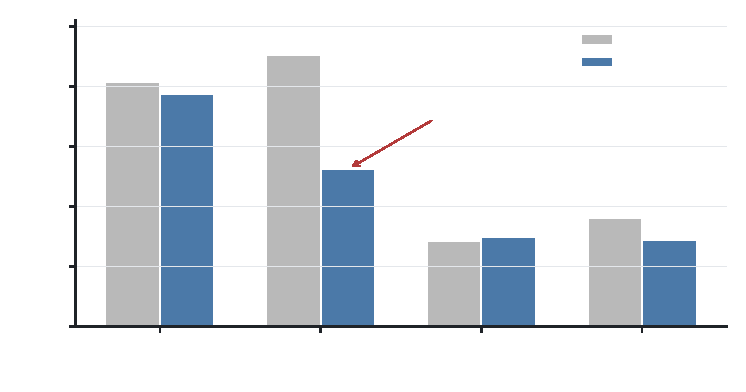
\includegraphics[width=0.85\textwidth]{figures/image5}
\caption{2WikiMultiHopQA per-type F1 (n=100, diagnostic). GERS-CV2 is close to CoT on comparison but lags on bridge\_comparison due to upstream entity error propagation; per-type sample counts are shown on the x-axis.}
\end{figure}

\begin{table}[h]
\centering
\caption{2WikiMultiHopQA per-type F1 (n=100)}
\begin{tabular}{lcccc}
\toprule
Method & comparison & bridge\_comp & compositional & inference \\
\midrule
Standard CoT & 0.815 & \textbf{0.905} & 0.284 & 0.361 \\
Zero-Shot & 0.800 & 0.587 & 0.366 & 0.330 \\
CoT-SC & 0.720 & 0.864 & 0.268 & 0.343 \\
GERS-CV2 & 0.775 & 0.524 & 0.297 & 0.288 \\
\bottomrule
\end{tabular}
\end{table}

\textbf{comparison}: GERS-CV2 F1=0.775, close to Standard CoT; the DAG naturally decomposes the two comparison branches. \textbf{bridge\_comparison}: GERS's clear weakness (0.524 vs 0.905); this ``bridge $\to$ compare $\to$ return to original entity'' composite question suffers from sub-question error propagation. Cross-validation raises bridge\_comparison F1 from 0.476 (without CV) to 0.524---partial mitigation but not a cure; the remaining gap stems from genuine reasoning error propagation, an inherent limitation of graph decomposition on deep multi-hop and a future direction.

\textbf{Boundary of graph-level self-consistency.} On 500 HotpotQA samples, GERS-SC (0.282) $\approx$ GERS+adaptive (0.284), $p=1.000$---multi-path selection yields no extra gain on medium-difficulty multi-hop even after fixing CS discrimination. Its value lies more in providing a quantifiable reasoning-quality signal.

\textbf{Why is Zero-Shot strong on HotpotQA?} Per-type breakdown (Table~\ref{tab:hpqa_type}) explains the anomaly: on \emph{bridge} questions (81\% of samples) all methods are close, as Qwen3-8B can extract answers directly from the context with little explicit reasoning; on \emph{comparison} questions, GERS-CV2 clearly beats both CoT-SC (+11.4pt EM) and Zero-Shot (+4.1pt EM), while CoT-SC falls below Zero-Shot---multi-sample voting adds noise on yes/no-style comparisons. Thus the structured method's advantage is concentrated on comparison/branch-merge samples, not uniformly across all questions. We further note that 2WikiMultiHopQA (n=100) serves as a \emph{diagnostic} boundary analysis rather than a main experiment; due to the limited size of per-type subsets, those results should be interpreted as indicative rather than definitive.

\begin{table}[h]
\centering
\caption{HotpotQA per-type EM (n=500).}
\label{tab:hpqa_type}
\begin{tabular}{lcc}
\toprule
Method & bridge (n=404) & comparison (n=96) \\
\midrule
Zero-Shot & 0.218 & 0.521 \\
CoT-SC & 0.218 & 0.448 \\
\textbf{GERS-CV2} & \textbf{0.240} & \textbf{0.562} \\
\bottomrule
\end{tabular}
\end{table}

\subsection{Computational Cost}

\begin{table}[h]
\centering
\caption{Cost comparison (HotpotQA, n=500, per-sample). LLM calls are estimated from the pipeline structure (1 decomposition + $n$ sub-steps + 1 aggregation, avg $n\approx2$; GERS-CV2 adds $n$ backward-verification calls).}
\resizebox{\linewidth}{!}{%
\begin{tabular}{lcccc}
\toprule
Method & LLM calls/q (est.) & Latency & EM & F1 \\
\midrule
Zero-Shot & 1 & 0.7s & 0.276 & 0.389 \\
Std CoT & 1 & 3.0s & 0.264 & 0.368 \\
CoT-SC (N=3) & 3 & 8.3s & 0.262 & 0.373 \\
GERS-Adap. & 1--4 & 4.8s & 0.284 & 0.395 \\
GERS-SC (K=3) & $\sim$12--15 & 16.2s & 0.282 & 0.398 \\
\textbf{GERS-CV2 (best)} & $\sim$6--8 & 6.6s & \textbf{0.302} & \textbf{0.413} \\
\bottomrule
\end{tabular}}
\end{table}

GERS-CV2 (single-path version) achieves the best EM=0.302 with $\sim$6--8 LLM calls and 6.6s latency. This uses more calls than CoT-SC's three samples, but remains comparable in wall-clock time under the parallel API setting, while leading by 4pt F1. The practical cost is moderated by adaptive routing (simple questions skip decomposition), shorter verification prompts, and backward verification only on complex questions. The multi-path GERS-SC ($\sim$12--15 calls) costs more with no performance gain, reinforcing the limited value of multi-path selection here.

\subsection{Ablation}

\begin{table}[h]
\centering
\caption{Ablation (HotpotQA, n=500)}
\begin{tabular}{lccl}
\toprule
Config & EM & F1 & Note \\
\midrule
GERS+adaptive & 0.284 & 0.395 & baseline: DAG + adaptive \\
GERS-SC (+K=3) & 0.282 & 0.398 & multi-path, old CS no discrimination \\
GERS-CV (+cross-validation) & 0.298 & 0.409 & new CS discriminative \\
\textbf{GERS-CV2 (+confidence)} & \textbf{0.302} & \textbf{0.413} & best \\
w/o graph execution (=CoT-SC+GERS) & 0.264 & 0.372 & no DAG execution \\
\bottomrule
\end{tabular}
\end{table}

\textbf{Cross-validation is the core gain source}: 0.284$\to$0.298, +1.4pt EM, corresponding to CS discrimination $-0.0035\to+0.0847$. \textbf{Graph-level self-consistency yields no extra gain}: GERS-SC $\approx$ GERS+adaptive, $p=1.000$ (a negative result). \textbf{Confidence weighting contributes marginally}: +0.4pt (not significant). \textbf{Graph execution is the foundation}: removing it degrades to 0.264.

\subsection{Case Study}

We illustrate how bidirectional verification distinguishes reasoning quality with two real HotpotQA samples (Table~\ref{tab:case}).

\textbf{Case A (self-consistent, correct).} Question: ``Were Scott Derrickson and Ed Wood of the same nationality?'' The forward pass decomposes into two sub-questions (nationality of each director), both yielding ``American'', leading to the correct answer ``yes''. Reverse verification, anchored on ``yes'' + context, independently re-derives both nationalities as ``American''---matching the forward answers. Crossval = 1.0, and the chain is retained.

\textbf{Case B (inconsistent, hallucination caught).} Question: ``Which director had the longest career, Alain Resnais or Scott Sidney?'' (gold: Scott Sidney). The forward pass confidently computes birth/death years (1922, 2014, 1902, 1975) and career lengths (92 vs 73 years), concluding ``Alain Resnais''---but these numbers are \emph{not present in the context} (the model hallucinated them). Reverse verification, re-deriving each sub-question from the context, repeatedly returns ``the context does not provide this information''---mismatching all 7 forward sub-answers. Crossval drops to 0.0, exposing the unsupported reasoning. Crucially, the old structural CS remains 0.7 (the DAG is legally connected and acyclic) and fails to detect the problem, whereas the new CS reflects the content inconsistency.

\begin{table}[h]
\centering
\caption{Real case study: forward vs.\ backward sub-answers.}
\label{tab:case}
\small
\begin{tabular}{p{2.2cm}p{3.2cm}p{3.2cm}p{1.3cm}p{1.1cm}p{1.1cm}}
\toprule
Case & Forward $a_i$ (excerpt) & Backward $a'_i$ (excerpt) & Match & Old CS & New CS \\
\midrule
A: nationalities & American / American & American / American & \checkmark & 1.0 & 1.0 \\
B: 7 sub-questions & 1922, 2014, 92yr, ... & ``not in context'' (all) & $\times$ & 0.7 & 0.0 \\
\bottomrule
\end{tabular}
\end{table}

The contrast is direct empirical evidence: when reasoning is grounded, forward and backward agree (New CS high); when the forward pass hallucinates facts absent from the context, backward verification detects the mismatch (New CS collapses) while the old structural CS stays inert.

\subsection{Generalization and Additional Ablations}

\textbf{Second model (generalization).} To check that the method is not specific to Qwen3-8B, we re-run on Qwen-Plus (a different, stronger model family) on 300 HotpotQA samples. GERS-CV2 (EM 0.363, F1 0.496) is on par with CoT-SC (EM 0.367, F1 0.494), diff $-0.004$, $p=1.000$. This indicates a generalization boundary: on a stronger base model, where Zero-Shot/CoT-SC already perform well, the structured method's advantage disappears. The gain is thus concentrated on medium-capability models where explicit decomposition matters.

\textbf{Weight design (P2.3).} Replacing the downstream-weighted $w_i$ with uniform weights yields EM 0.300 / F1 0.411 (vs.\ 0.302 / 0.413), indistinguishable. The weighting design does not affect end performance; it is kept for interpretability.

\textbf{Anchor ablation (P2.4).} A context-only backward verification (no final-answer anchor) achieves EM 0.300 / F1 0.414---matching the default---while the CS drops to 0.646 (vs.\ 0.777), showing the verification is stricter without the anchor and the performance does not rely on the final answer as an anchor.

\textbf{2Wiki at larger scale (P2.1).} Extending 2WikiMultiHopQA to 300 samples confirms the boundary: GERS-CV2 EM 0.390 remains below Standard CoT 0.443, with the gap concentrated on bridge\_comparison. The larger sample makes the diagnostic boundary more reliable.

\section{Discussion and Limitations}

\textbf{Core value of bidirectional verification.} The main contribution is raising CS discrimination from $-0.0035$ to $+0.0847$, upgrading consistency checking from ``is the graph legal'' to ``is the reasoning content self-consistent''. This verification is naturally supported by explicit DAG decomposition. The EM gain (+1.4pt) is modest, but the mechanism's effectiveness and quantifiable evidence are clear.

\textbf{Confirmation bias of reverse verification.} Anchoring backward re-derivation on the final answer $A$ can bias the model toward explanations consistent with $A$, risking spurious agreement. We mitigate this by instructing the model to derive from the context rather than copy $A$. We also ran a context-only control (Section~4.8) where backward verification uses no final answer: performance is unchanged (EM 0.300) while the CS drops to 0.646 (stricter), indicating the gain does not depend on the $A$-anchor and the bias is limited. Adversarial-answer perturbation remains future work.

\textbf{Self-consistency is not correctness.} A key limitation exposed by our negative repair experiments is that raising the cross-validation score can make a reasoning chain more internally self-consistent without necessarily making it more correct. This suggests that bidirectional verification should be interpreted as a content-consistency signal, not as a complete correctness verifier. The missing ingredient is \emph{evidence grounding}: each forward/backward sub-answer should be supported by an explicit context span. Without this external grounding, a model can still produce a coherent but unsupported reasoning chain. We therefore view evidence-grounded verification as the next step toward turning GERS-CV from a diagnostic signal into a reliable repair mechanism.

\textbf{Honest positioning.} GERS-CV2 is McNemar-significant on EM correctness ($p=0.029$) but the paired bootstrap effect-size CIs marginally cross zero---``paired-significant on correctness, effect-size marginal''. A key reason for the limited overall gain: HotpotQA's context directly contains answer evidence, so Zero-Shot (0.276) is already close to GERS, compressing the advantage of structured methods.

\textbf{Boundary of graph-level self-consistency.} Even after fixing CS discrimination, $K=3$ multi-path selection yields no extra gain on medium-difficulty multi-hop ($p=1.000$); single-path DAG execution suffices, and multi-path selection is redundant.

\textbf{Deep bridging limitation.} On bridge\_comparison, GERS's error propagation lags behind linear CoT, an inherent limitation of graph decomposition on deep multi-hop.

\textbf{Comparison with existing graph methods.} Unlike MoDeGraph et al.\ which use the graph only as context, GERS's graph participates in both execution and content checking, forming a ``decompose--execute--check'' closed loop.

\section{Conclusion}

We propose GERS, whose core innovation is \textbf{bidirectional sub-answer verification}: using the final answer and context as an anchor to re-derive sub-questions in reverse and compare forward/backward consistency, upgrading the Consistency Score from a pure graph-theoretic metric (discrimination $-0.0035$, providing little discriminative signal) to an effective content self-consistency signal (discrimination $+0.0847$). This verification is naturally supported by explicit DAG decomposition. The best configuration GERS-CV2 achieves EM=0.302, F1=0.413 on 500 HotpotQA samples, with a significant McNemar test on EM correctness against CoT-SC ($p=0.029$) and a +4pt F1 difference, but marginal paired bootstrap effect-size intervals that we report transparently. We also provide a boundary analysis showing the method suits comparison-style decomposition but fails on deep bridge-comparison questions, and note that engineering fixes (metric, extraction, answer-type) are necessary to avoid format-induced errors being mistaken for reasoning errors.

Future work: (1) incorporate evidence-grounded verification so that each sub-answer is checked against explicit context spans, not only against reverse self-consistency; (2) design conservative local re-generation for deep bridging-comparison to mitigate error propagation without overwriting correct intermediate answers; (3) validate cross-validation on larger models and more datasets.

\begin{thebibliography}{99}
\bibitem{wei2022cot} Wei, J., et al. Chain-of-Thought Prompting Elicits Reasoning in Large Language Models. In \emph{NeurIPS}, 2022.
\bibitem{besta2024got} Besta, M., et al. Graph of Thoughts: Solving Elaborate Problems with Large Language Models. In \emph{AAAI}, 2024.
\bibitem{han2025rwg} Han, H., et al. Reasoning with Graphs: Structuring Implicit Knowledge to Enhance LLMs Reasoning. In \emph{Findings of ACL}, 2025.
\bibitem{oruche2025modegraph} Oruche, R., et al. Disentangling Complex Questions in LLMs via Multi-Hop Dependency Graphs. In \emph{CIKM}, 2025.
\bibitem{ni2025stepchain} Ni, T., et al. StepChain GraphRAG: Reasoning Over Knowledge Graphs for Multi-hop Question Answering. \emph{arXiv:2510.02827}, 2025.
\bibitem{wang2023sc} Wang, X., et al. Self-Consistency Improves Chain of Thought Reasoning in Language Models. In \emph{ICLR}, 2023.
\bibitem{yao2023tot} Yao, S., et al. Tree of Thoughts: Deliberate Problem Solving with Large Language Models. In \emph{NeurIPS}, 2023.
\bibitem{lightman2024verify} Lightman, H., et al. Let's Verify Step by Step. In \emph{ICLR}, 2024.
\bibitem{madaan2023selfrefine} Madaan, A., et al. Self-Refine: Iterative Refinement with Self-Feedback. In \emph{NeurIPS}, 2023.
\bibitem{yang2018hotpotqa} Yang, Z., et al. HotpotQA: A Dataset for Diverse, Explainable Multi-hop Question Answering. In \emph{EMNLP}, 2018.
\bibitem{ho20202wiki} Ho, X., et al. Constructing A Multi-hop QA Dataset for Comprehensive Evaluation of Reasoning Steps. In \emph{COLING}, 2020.
\end{thebibliography}

\end{document}
